\begin{samplecase}
{\bf Spherical optical model and DWBA: n + ${}^{208}$Pb}\newline

Three types of optical model calculations are included in the set of sample
cases. In this first one, we treat ${}^{208}$Pb as a spherical nucleus and
request calculations for the elastic angular
distributions and inelastic angular distributions at a few incident energies.
This is accomplished with the input file

\VerbatimInput{\samples n-Pb208-omp/org/talys.inp}

where the file {\em energies} consists of the energies 11., 13.7, 20., 22.,
and 25.7 MeV (for which experimental data exists). The keyword
{\em fileelastic y} has created the files {\em nn011.000ang.L00}, etc. which
contain the elastic scattering angular distribution and are compared with
experimental data in Fig.~\ref{pbdwba}.
With {\bf fileangle 1} and {\bf fileangle 2} we have created the files
{\em nn010.000ang.L01}, etc.  with the inelastic scattering angular
distribution to the first and second discrete state.
These are also plotted in Figs.~\ref{pbdwba}.
Note that the keywords in the middle block ({\bf ejectiles n} up to
{\bf filetotal n}) have been added to avoid a full calculation of all the
cross sections. For the present sample case we assume that only elastic
scattering and DWBA angular distributions are
of interest, so we economize on output options, number of bins, ejectiles and
nuclides that can be reached. Obviously, for reliable results for all
observables this middle block would have to be deleted.
See also sample case (1f) for obtaining more specific information from the
output.

\end{samplecase}
\begin{figure}
\centerline{
\centering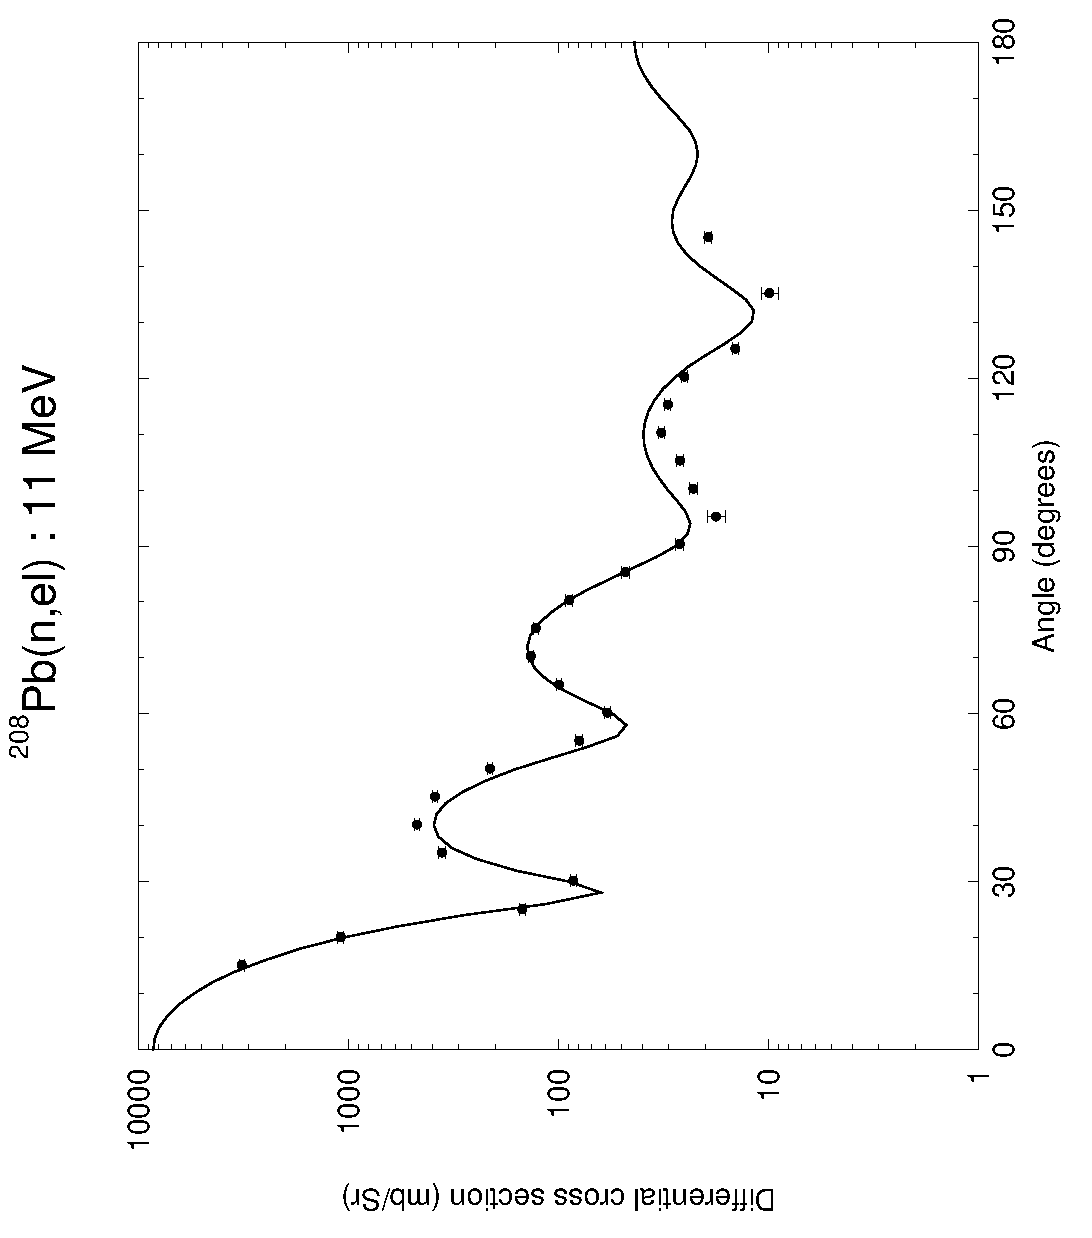
\includegraphics[scale=0.3,angle=270]{el11} \centering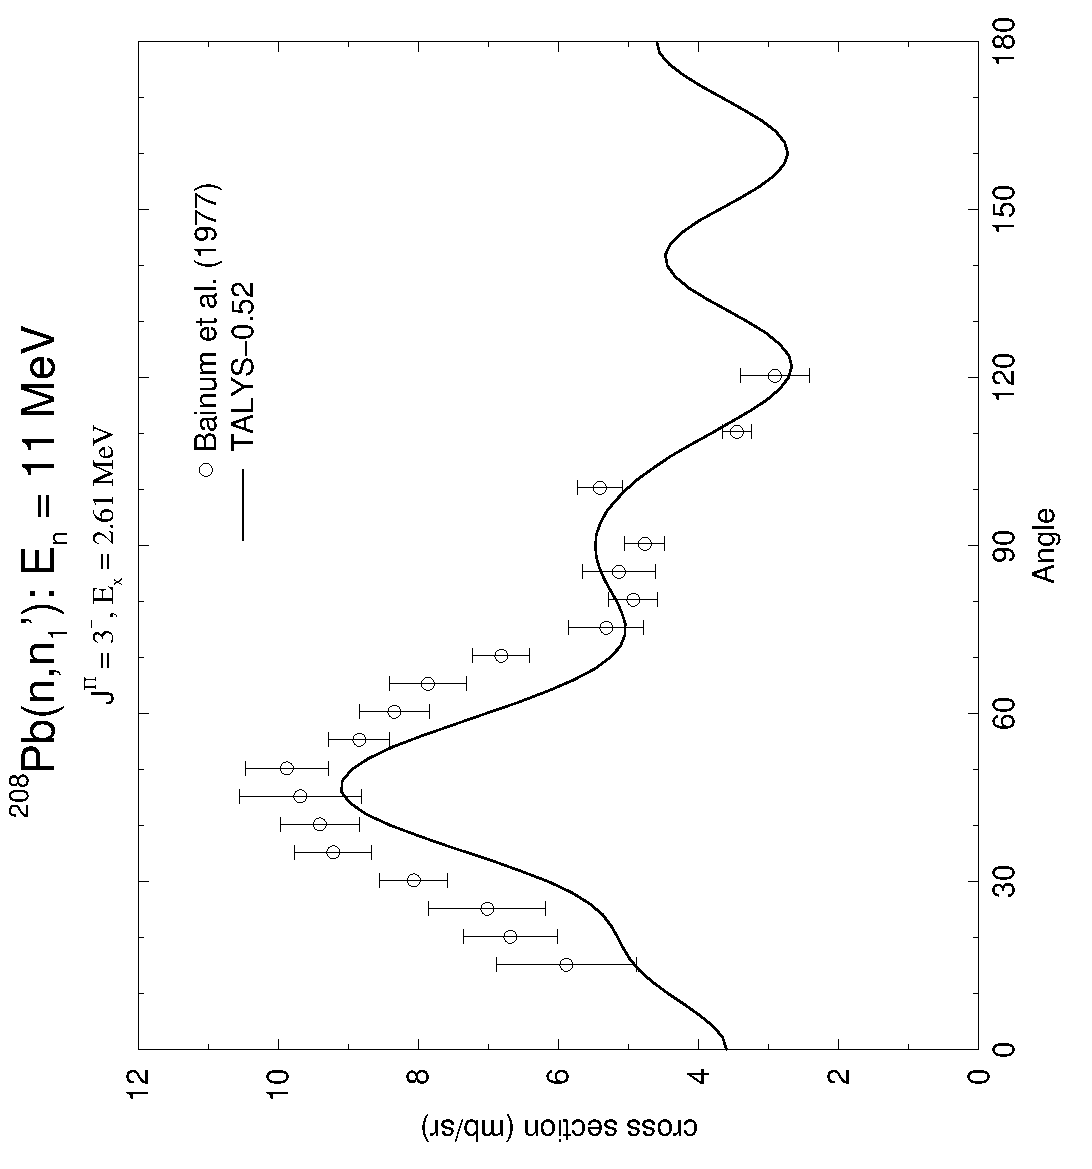
\includegraphics[scale=0.3,angle=270]{in1e11} \centering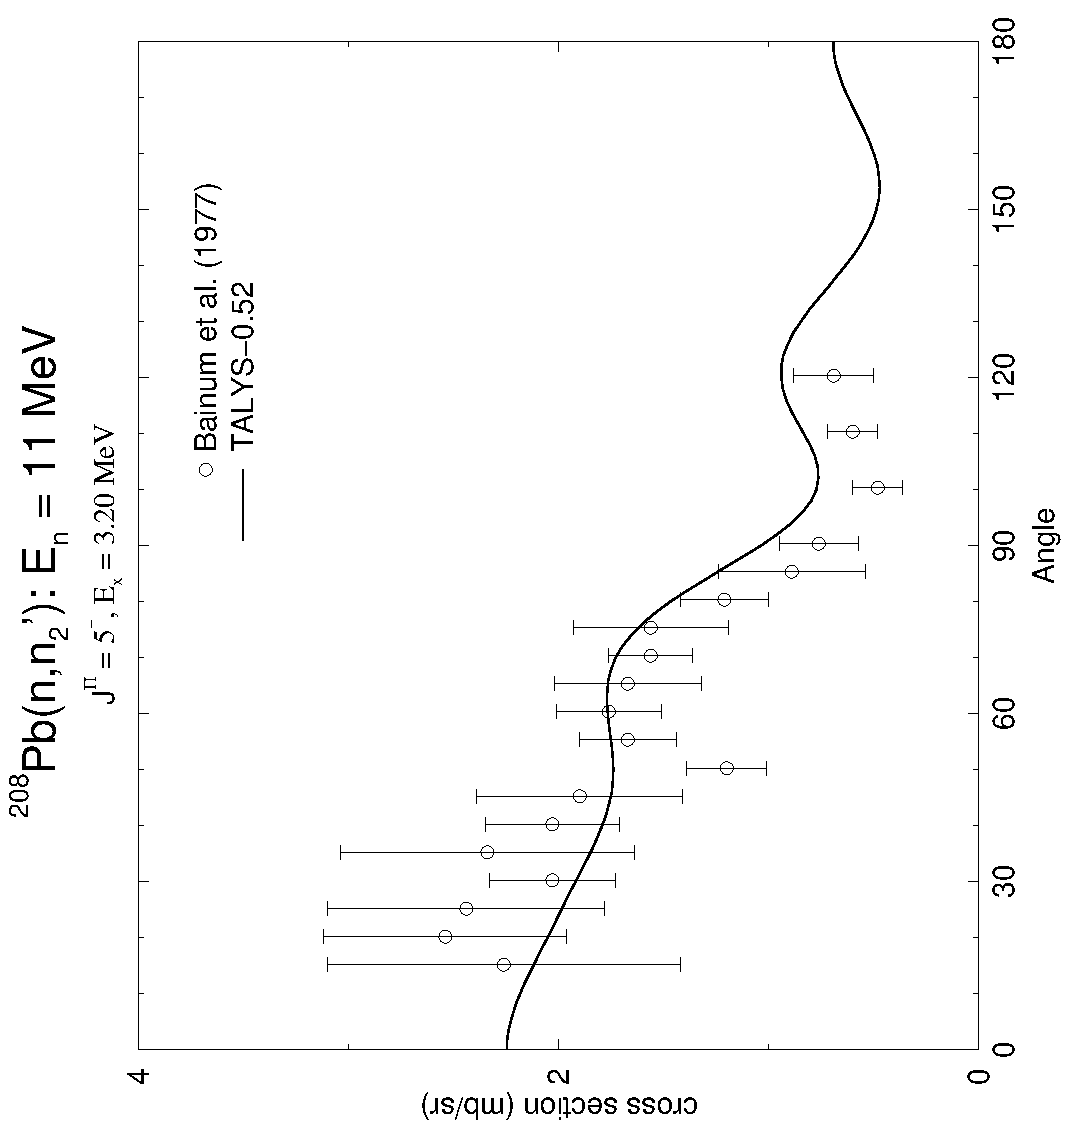
\includegraphics[scale=0.3,angle=270]{in2e11}
}
\centerline{
\centering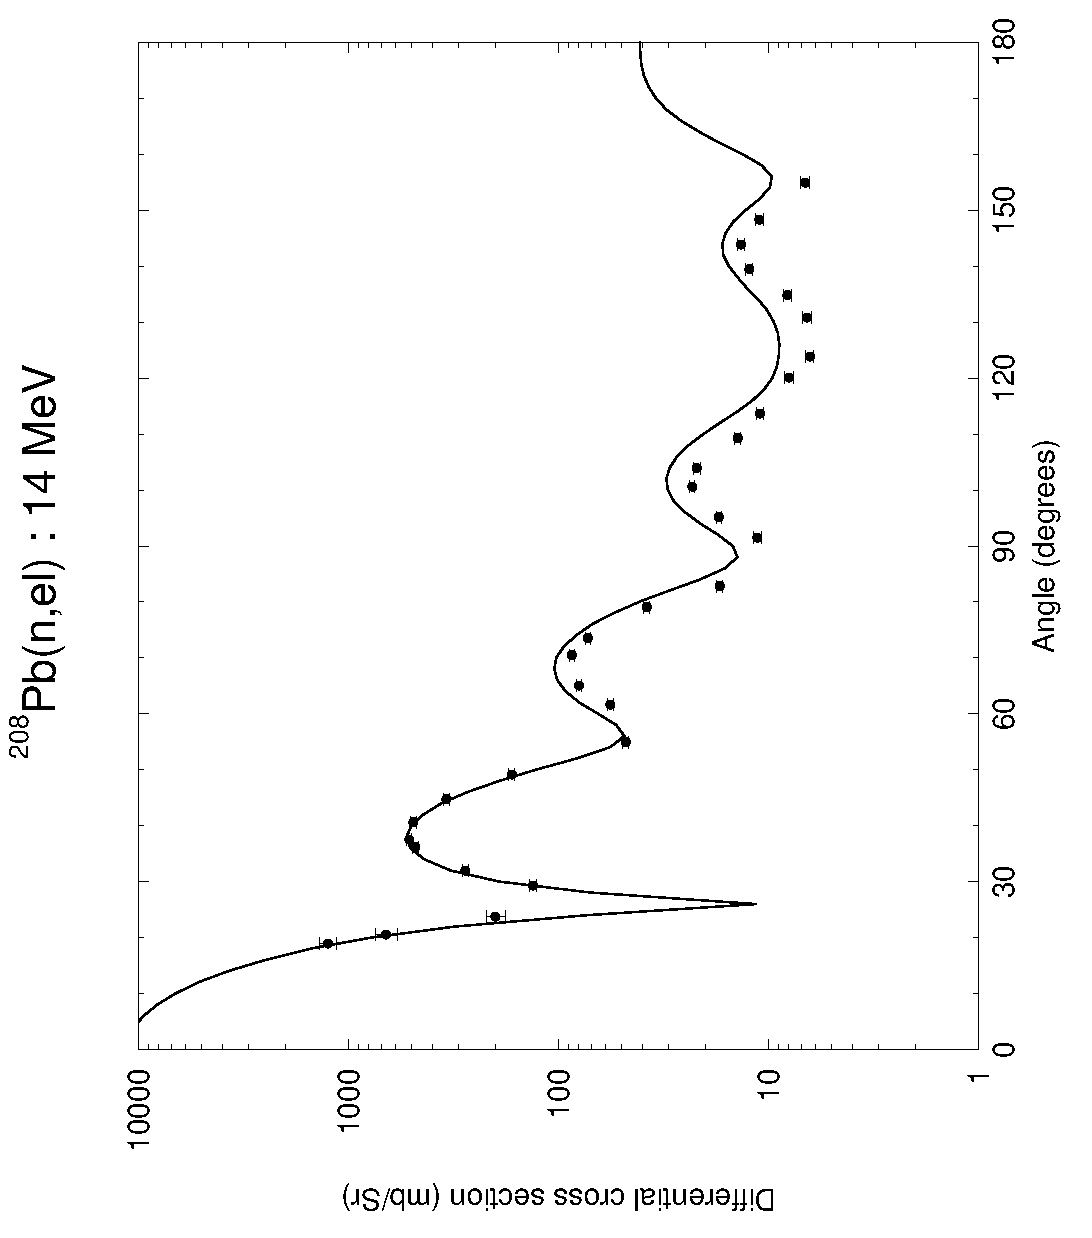
\includegraphics[scale=0.3,angle=270]{el14} \centering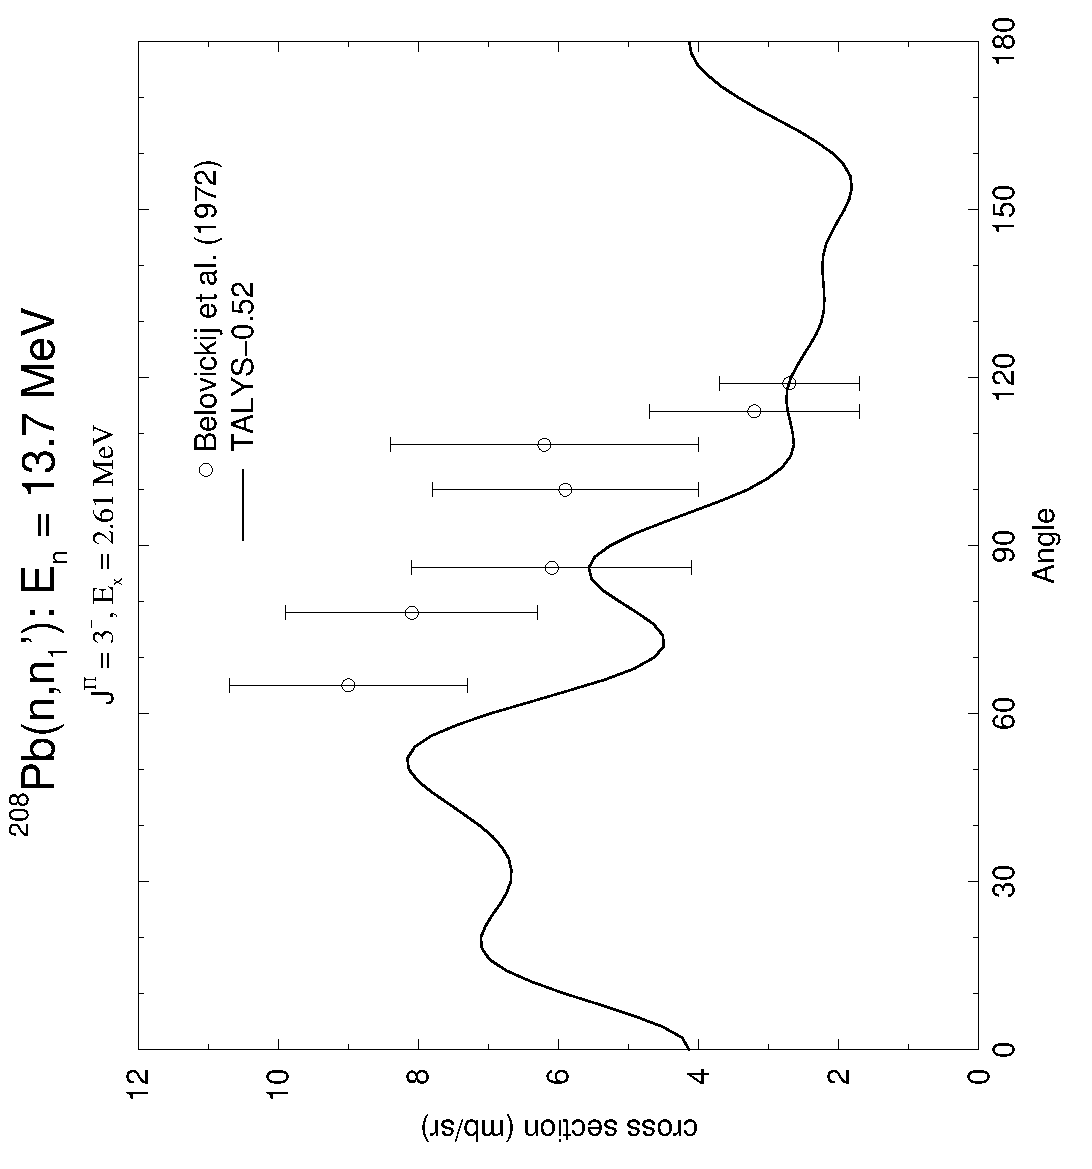
\includegraphics[scale=0.3,angle=270]{in1e14} \centering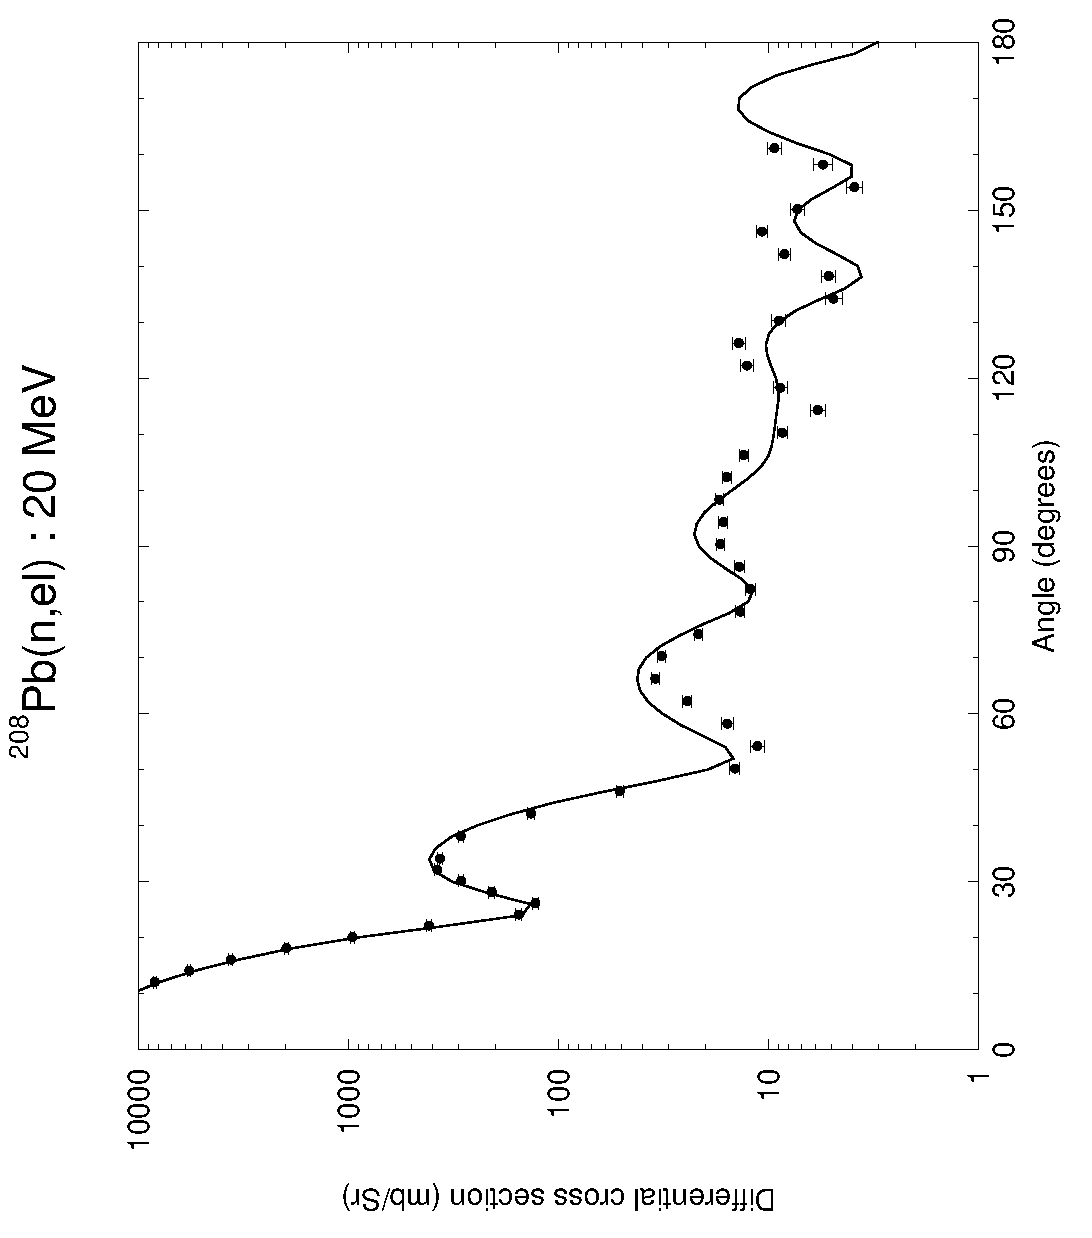
\includegraphics[scale=0.3,angle=270]{el20}
}
\centerline{
\centering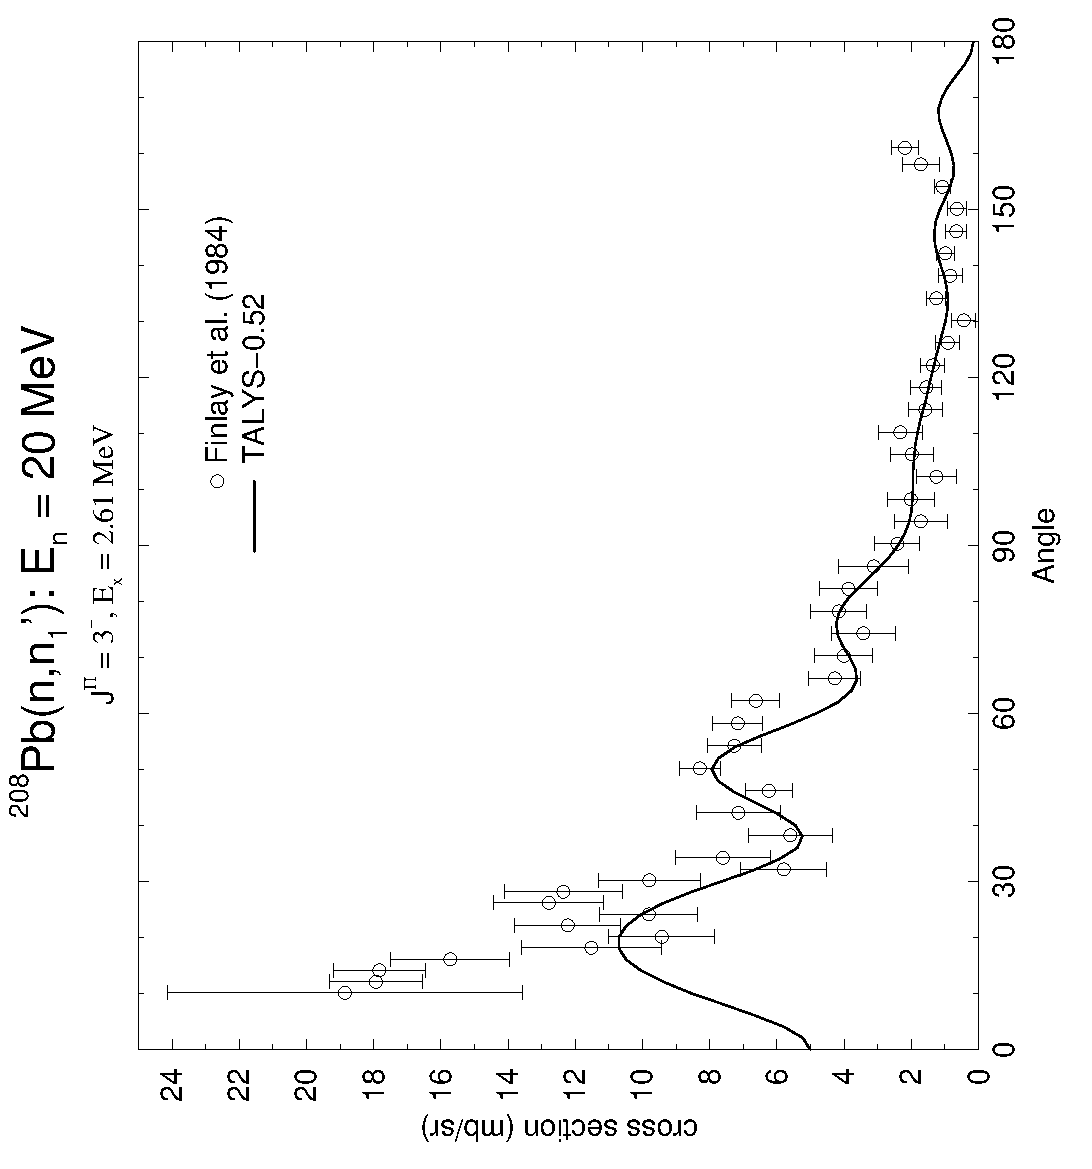
\includegraphics[scale=0.3,angle=270]{in1e20} \centering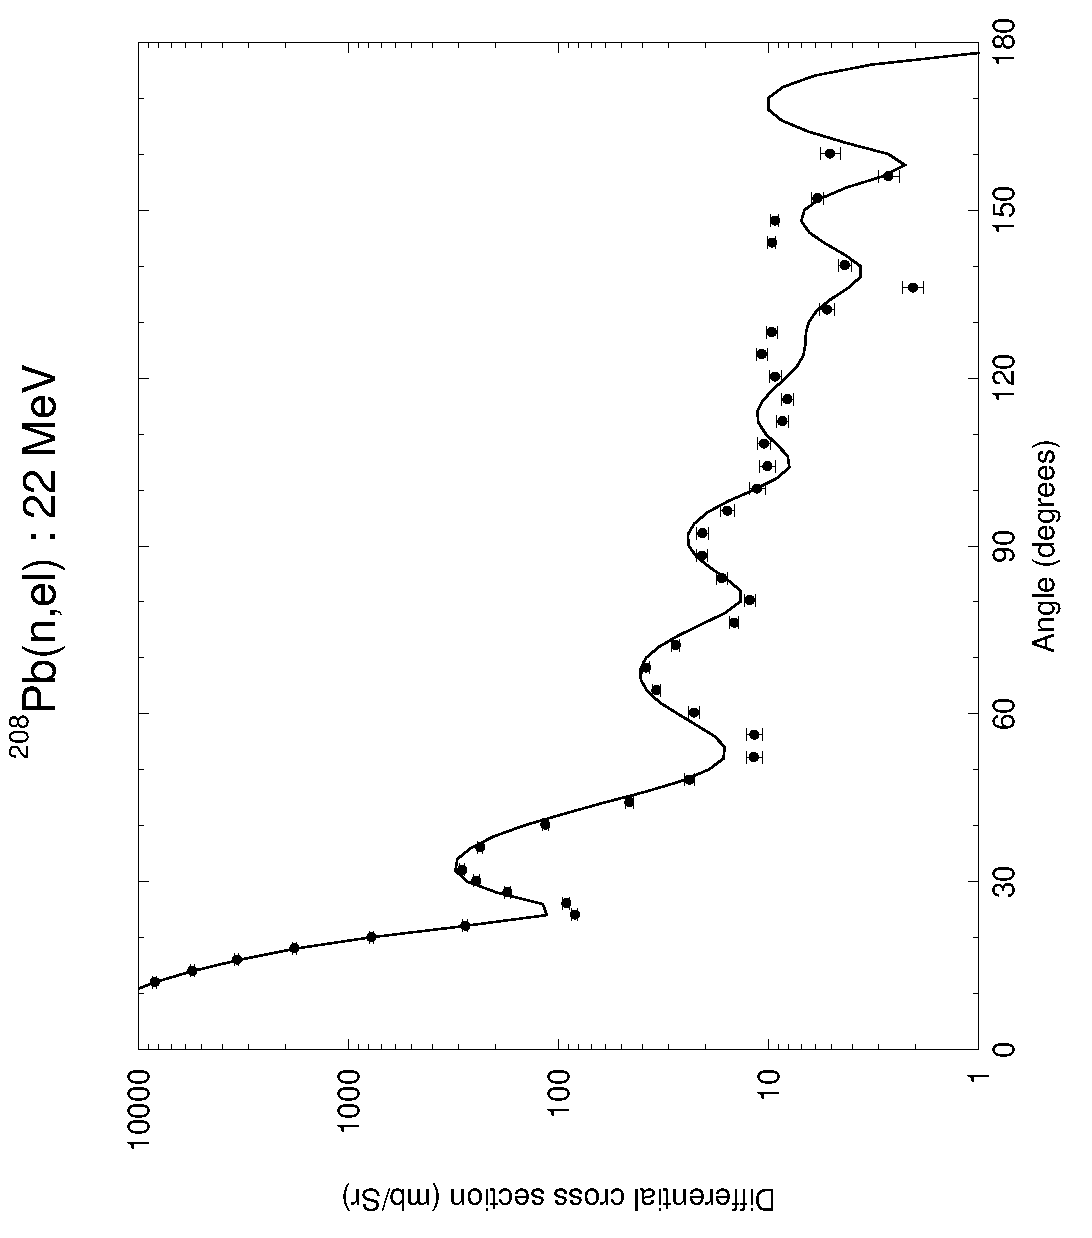
\includegraphics[scale=0.3,angle=270]{el22} \centering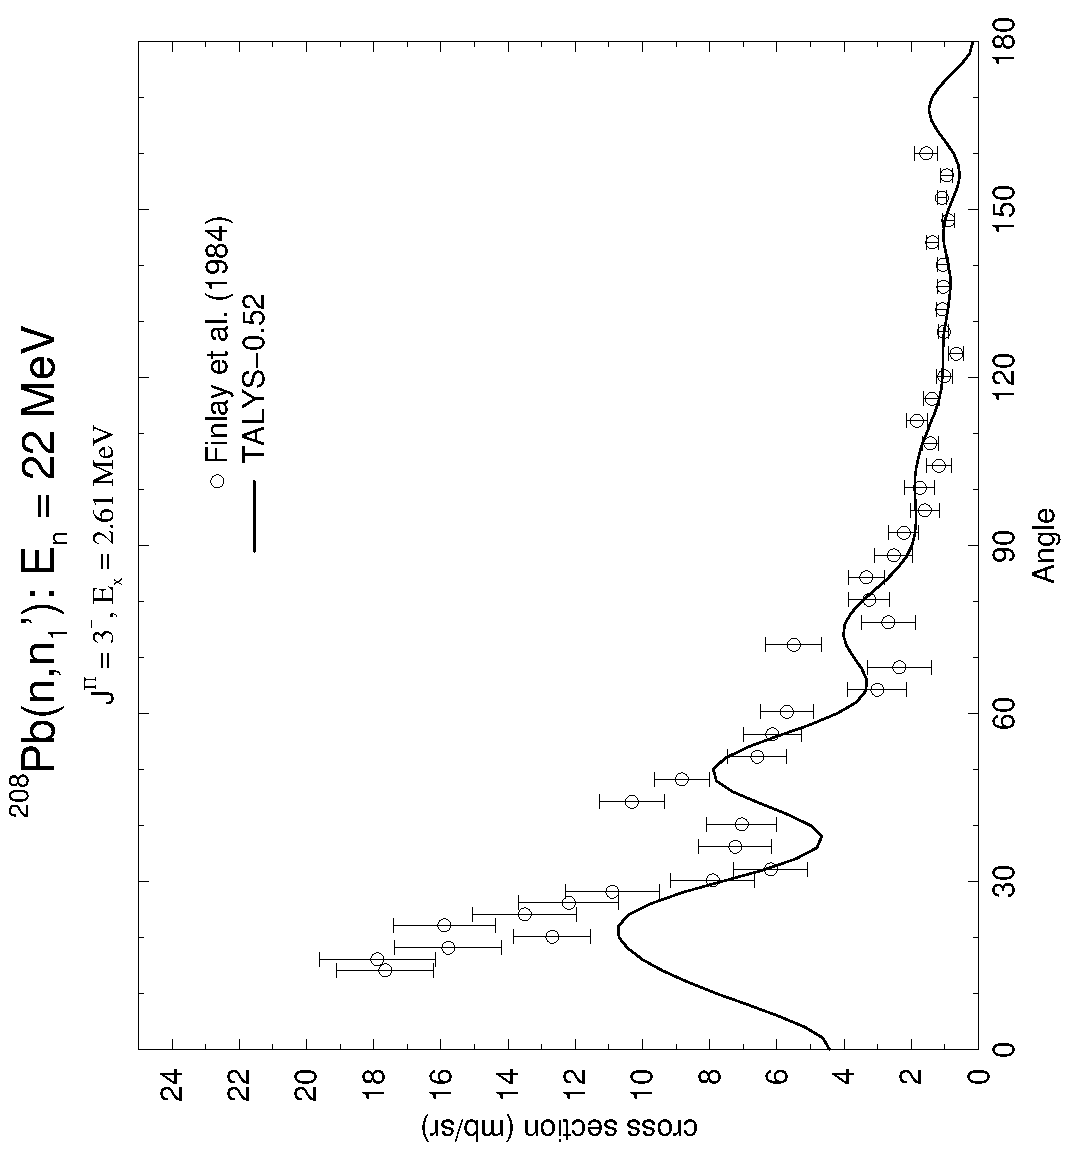
\includegraphics[scale=0.3,angle=270]{in1e22}
}
\centerline{
\centering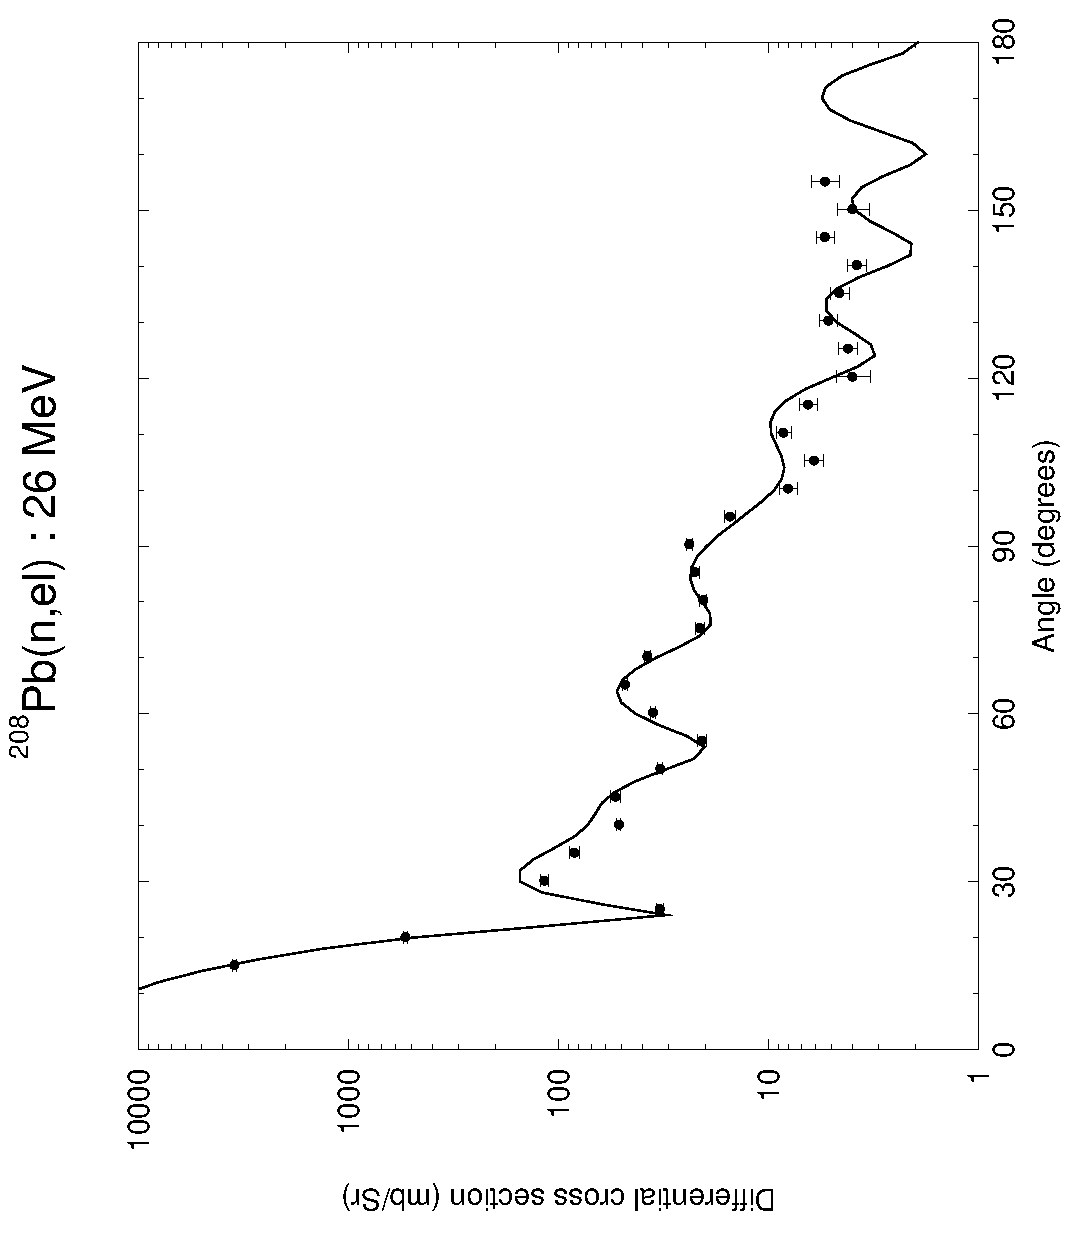
\includegraphics[scale=0.3,angle=270]{el26} \centering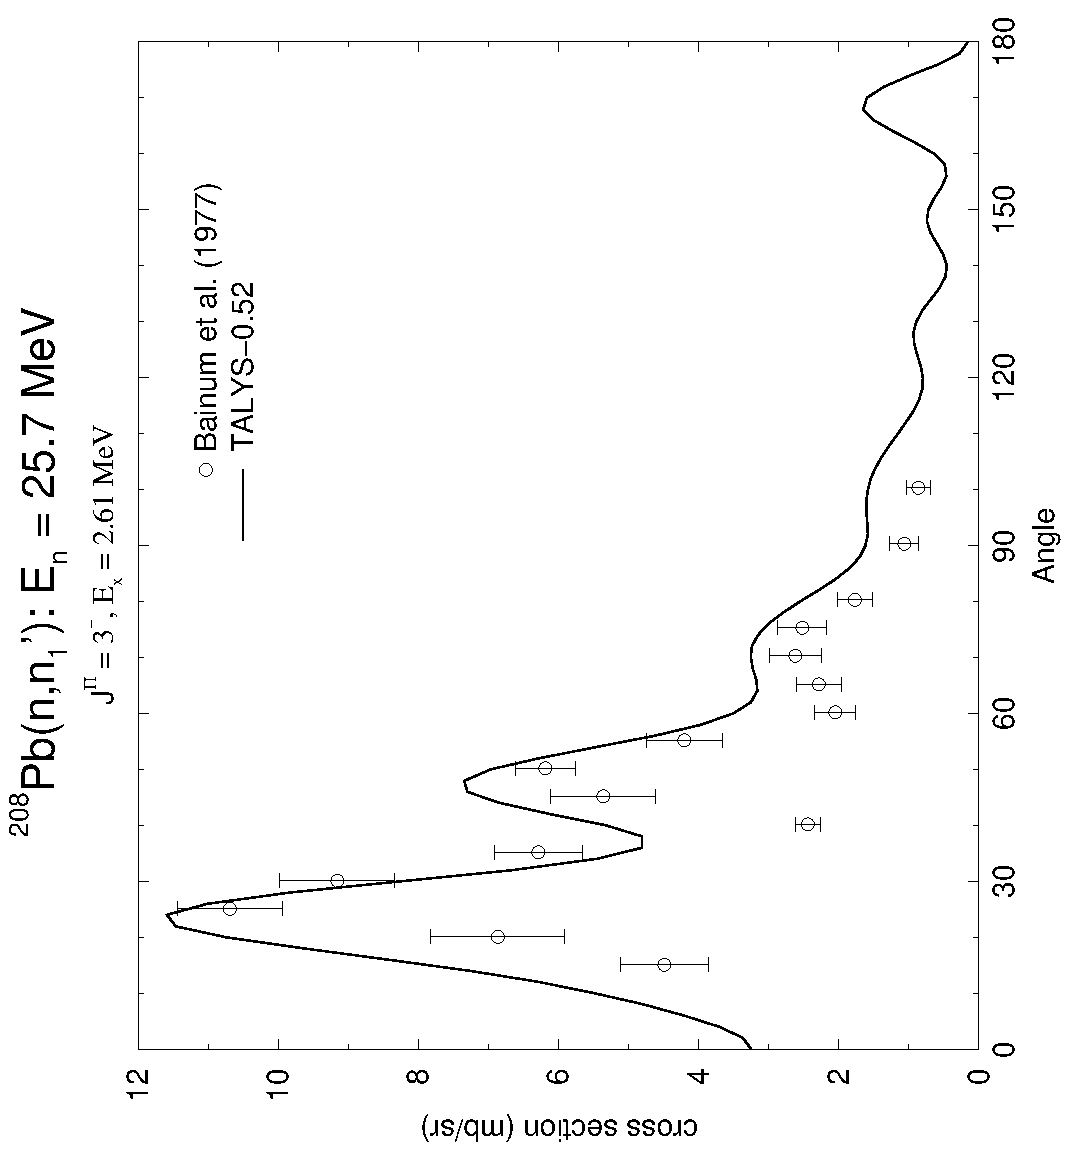
\includegraphics[scale=0.3,angle=270]{in1e26} \centering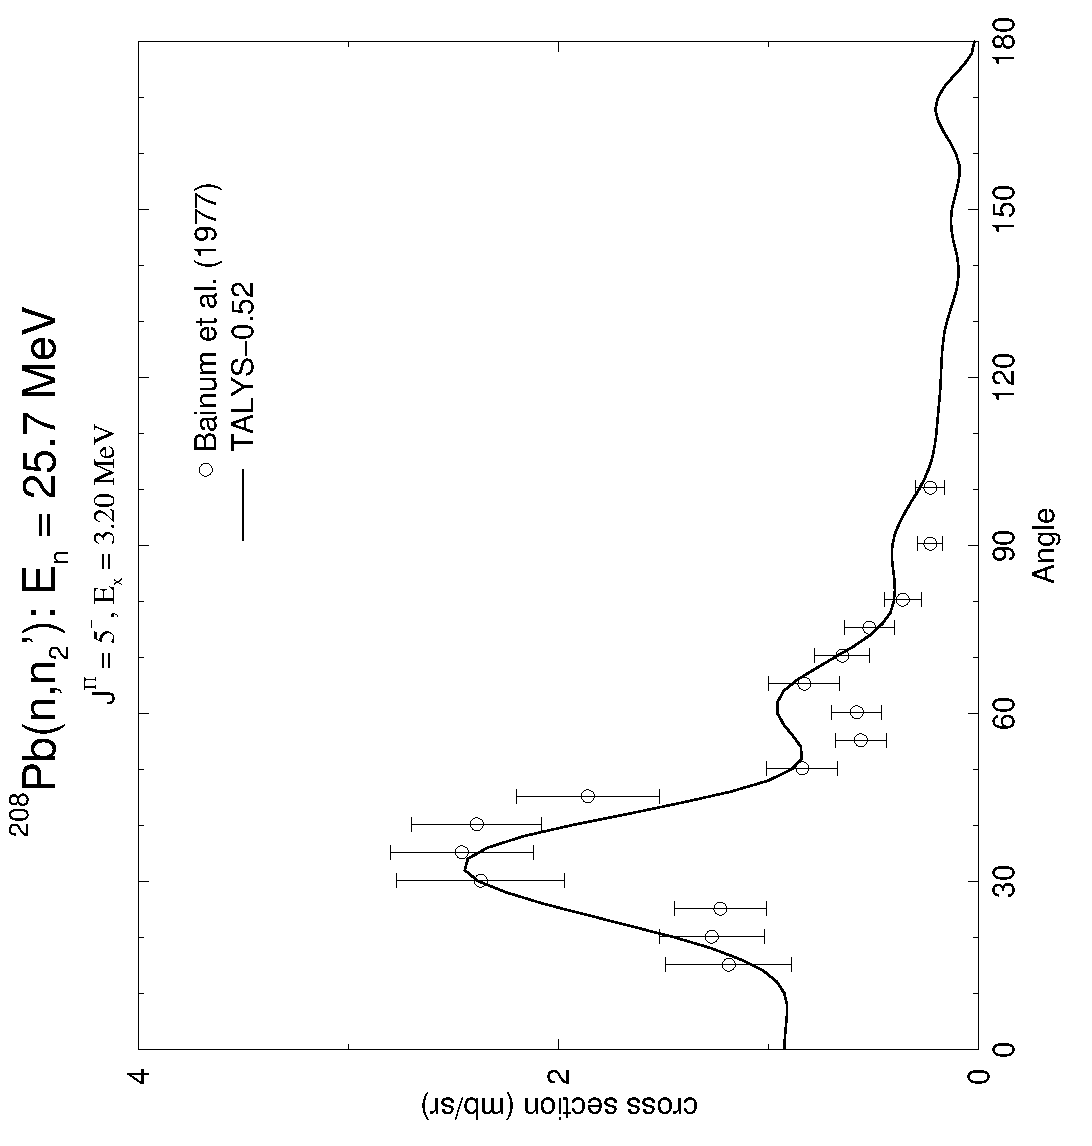
\includegraphics[scale=0.3,angle=270]{in2e26}
}
\caption{Elastic and inelastic scattering angular distributions between
11 and 26 MeV for ${}^{208}$Pb.}
\label{pbdwba}
\end{figure}
